\documentclass{beamer}
\usepackage{graphicx}
\usepackage{verbatim}
\usepackage{xcolor}
\usepackage{colortbl}

\renewcommand{\figurename}{Gambar}
\renewcommand{\tablename}{Tabel}

\usetheme{metropolis}
\setbeamertemplate{navigation symbols}{}
\usepackage{listings}
\usepackage{xcolor}
\usepackage{ragged2e}
\usepackage{url}

\definecolor{codegreen}{rgb}{0,0.6,0}
\definecolor{codegray}{rgb}{0.5,0.5,0.5}
\definecolor{codepurple}{rgb}{0.58,0,0.82}
\definecolor{backcolour}{rgb}{0.95,0.95,0.92}

\lstset{
    language=Java,
    backgroundcolor=\color{backcolour},   
    commentstyle=\color{codegreen},
    keywordstyle=\color{magenta},
    numberstyle=\tiny\color{codegray},
    stringstyle=\color{codepurple},
    basicstyle=\ttfamily\footnotesize,
    breakatwhitespace=false,         
    breaklines=true,                 
    captionpos=b,                    
    keepspaces=true,                 
    numbers=left,                    
    numbersep=5pt,                  
    showspaces=false,                
    showstringspaces=false,
    showtabs=false,                  
    tabsize=2,
    frame=single,
    columns=flexible
}

\addtobeamertemplate{block begin}{}{\justifying}
\addtobeamertemplate{block begin}{}{\vspace{3px}}

% Info presentasi
\title{Algoritma dan Pemrograman Komputer 1}
\subtitle{Bab 7: Perulangan (Looping)}
\author{Aslam Pandu Tasminto -- 5002241025 \\ M. Ma'ruf Qomaruddin Kafi -- 5002241095}
\date{October 20, 2025}
\institute{Departemen Matematika \\ Fakultas Sains dan Analitika Data \\ Institut Teknologi Sepuluh Nopember}

% Logo untuk title page
\titlegraphic{%
  
\includegraphics[height=0.9cm]{../assets/logoprovikom.jpg}%
  \hspace{0.5em}%
  
\includegraphics[height=0.9cm]{../assets/logomatematika.png}%
  \hspace{0.5em}%
  
\includegraphics[height=1cm]{../assets/logoits.png}%
}

\begin{document}

% Cover
\maketitle

% Daftar Isi
\begin{frame}{Daftar Isi}
  \tableofcontents
\end{frame}

% Section 1: Pengenalan Perulangan
\section{Pengenalan Perulangan}
\begin{frame}{Konsep Perulangan dalam Java}
  \begin{block}{Definisi}
    Perulangan (looping) adalah struktur kontrol yang digunakan untuk mengeksekusi blok kode secara berulang-ulang selama kondisi tertentu terpenuhi.
  \end{block}
  \begin{block}{Jenis Perulangan dalam Java}
    \begin{itemize}
      \item \texttt{for} loop - ketika jumlah perulangan diketahui
      \item \texttt{while} loop - ketika jumlah perulangan tidak pasti
      \item \texttt{do-while} loop - minimal 1x eksekusi dijamin
    \end{itemize}
  \end{block}
  \begin{block}{Manfaat Perulangan}
    \begin{itemize}
      \item Mengurangi duplikasi kode
      \item Efisiensi dalam penulisan program
      \item Memudahkan proses iterasi data
    \end{itemize}
  \end{block}
\end{frame}

% Section 2: FOR Loop
\section{FOR Loop}
\begin{frame}[fragile]{Sintaks dan Struktur FOR Loop}
  \begin{block}{Struktur Dasar FOR Loop}
    \begin{lstlisting}
for (inisialisasi; kondisi; perubahan) {
    // pernyataan yang diulang
}
    \end{lstlisting}
  \end{block}
  
  \begin{table}
    \footnotesize
    \begin{tabular}{p{0.25\textwidth}|p{0.65\textwidth}}
    \textbf{Komponen} & \textbf{Deskripsi} \\
    \hline
    \rowcolor{lightgray}
    \texttt{inisialisasi} & Inisialisasi variabel counter (contoh: \texttt{int i = 0}) \\
    \rowcolor{white}
    \texttt{kondisi} & Kondisi untuk melanjutkan perulangan (contoh: \texttt{i < 5}) \\
    \rowcolor{lightgray}
    \texttt{perubahan} & Perubahan nilai counter tiap iterasi (contoh: \texttt{i++}) \\
    \rowcolor{white}
    \texttt{pernyataan} & Blok kode yang dieksekusi berulang kali \\
    \end{tabular}
    \caption{Komponen-komponen dalam FOR Loop}
  \end{table}
\end{frame}

\begin{frame}[fragile]{Contoh FOR Loop Sederhana}
  \begin{exampleblock}{Contoh Program FOR Loop Dasar}
    \begin{lstlisting}
public class ForLoop {
    public static void main(String[] args) {
        // Menampilkan "Selamat datang" 5 kali
        for (int i = 0; i < 5; i++) {
            System.out.println("Selamat datang");
        }
    }
}
    \end{lstlisting}
  \end{exampleblock}
  
  \vspace{-0.5cm} 
  
  \textbf{Output Program}
    \colorbox{gray!20}{
      \parbox{0.9\textwidth}{
        {\footnotesize
        \texttt{Selamat datang\\
        Selamat datang\\
        Selamat datang\\
        Selamat datang\\
        Selamat datang}
        }
      }
    }
\end{frame}

\begin{frame}[fragile]{Variasi FOR Loop}
  \begin{exampleblock}{FOR Loop dengan Pola Berbeda}
    \begin{lstlisting}[basicstyle=\ttfamily\scriptsize]
public class ForVariasi {
    public static void main(String[] args) {
        // Decrement
        for(int i = 5; i > 0; i--) {
            System.out.println(i);
        }
        
        // Kelipatan 2
        for(int j = 0; j < 10; j = j + 2) {
            System.out.println(j);
        }
        
        // Perkalian
        for(int k = 1; k < 17; k = k * 2) {
            System.out.println(k);
        }
    }
}
    \end{lstlisting}
  \end{exampleblock}
\end{frame}

\begin{frame}[fragile]{Flowchart FOR Loop}
  \begin{figure}
    \centering
    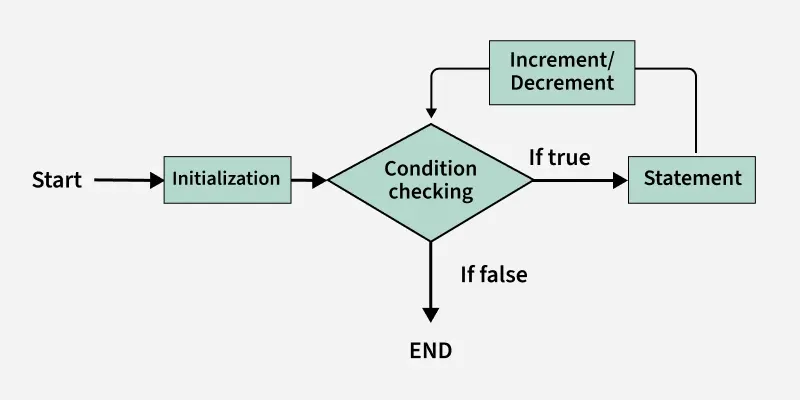
\includegraphics[width=0.75\linewidth]{Perulangan/for_loop_flowchart.png}
    \caption{Alur eksekusi FOR Loop dalam Java}
    \label{fig:placeholder}
\end{figure}
  \textbf{Sumber: }GeeksforGeeks - Java Loops
\end{frame}

% Section 3: WHILE Loop
\section{WHILE Loop}
\begin{frame}[fragile]{Sintaks dan Struktur WHILE Loop}
  \begin{block}{Struktur Dasar WHILE Loop}
    \begin{lstlisting}
while (kondisi) {
    // pernyataan yang diulang
}
    \end{lstlisting}
  \end{block}

  \vspace{-0.2cm}
  
  \begin{table}
    \scriptsize
    \begin{tabular}{p{0.25\textwidth}|p{0.65\textwidth}}
    \textbf{Komponen} & \textbf{Deskripsi} \\
    \hline
    \rowcolor{lightgray}
    \texttt{kondisi} & Ekspresi boolean yang dievaluasi sebelum setiap iterasi \\
    \rowcolor{white}
    \texttt{pernyataan} & Blok kode yang dieksekusi berulang selama kondisi true \\
    \end{tabular}
    \caption{Komponen-komponen dalam WHILE Loop}
  \end{table}

  \vspace{-0.2cm}
  
  \begin{block}{Karakteristik WHILE Loop}
  \scriptsize
    \begin{itemize}
      \item Kondisi diperiksa \textbf{sebelum} eksekusi blok pernyataan
      \item Jika kondisi false sejak awal, blok tidak akan dieksekusi sama sekali
      \item Cocok untuk kasus dimana jumlah iterasi tidak diketahui
      \item Pastikan ada mekanisme untuk mengubah kondisi atau akan terjadi \textbf{infinite loop}!
    \end{itemize}
  \end{block}
  
  
\end{frame}


\begin{frame}[fragile]{Contoh WHILE Loop}
\vspace{-0.2cm}
  \begin{exampleblock}{Contoh Program WHILE Loop}
    \begin{lstlisting}[basicstyle=\ttfamily\scriptsize]
public class WhileLoop {
    public static void main(String[] args) {
        int i = 0;
        
        // Menampilkan "Selamat datang" 5 kali
        while (i < 5) {
            System.out.println("Selamat datang");
            i++;  // Jangan lupa increment!
        }
    }
}
    \end{lstlisting}
  \end{exampleblock}

  \vspace{-0.6cm}
  \textbf{Output Program}
    \colorbox{gray!20}{
      \parbox{0.9\textwidth}{
        {\scriptsize
        \texttt{Selamat datang\\
        Selamat datang\\
        Selamat datang\\
        Selamat datang\\
        Selamat datang}
        }
      }
    }

\end{frame}

\begin{frame}{Flowchart WHILE Loop}
  \begin{figure}
      \centering
      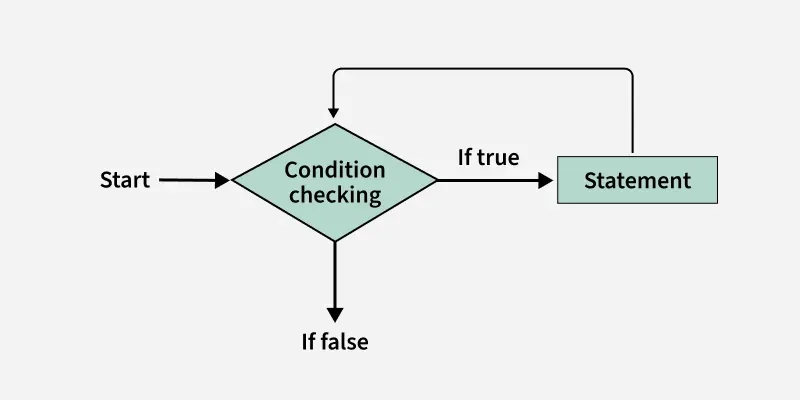
\includegraphics[width=0.75\linewidth]{Perulangan/while_loop_flowchart.png}
      \caption{Alur eksekusi WHILE Loop dalam Java}
      \label{fig:placeholder}
  \end{figure}
  \textbf{Sumber: }GeeksforGeeks - Java Loop
\end{frame}

% Section 4: DO-WHILE Loop
\section{DO-WHILE Loop}
\begin{frame}[fragile]{Sintaks dan Struktur DO-WHILE Loop}
  \begin{block}{Struktur Dasar DO-WHILE Loop}
    \begin{lstlisting}
do {
    // pernyataan yang diulang
} while (kondisi);
    \end{lstlisting}
  \end{block}
  
  \vspace{-0.3cm}
  \begin{table}
    \footnotesize
    \begin{tabular}{p{0.25\textwidth}|p{0.65\textwidth}}
    \textbf{Komponen} & \textbf{Deskripsi} \\
    \hline
    \rowcolor{lightgray}
    \texttt{do} & Keyword yang menandai awal blok pernyataan \\
    \rowcolor{white}
    \texttt{pernyataan} & Blok kode yang dieksekusi minimal sekali \\
    \rowcolor{lightgray}
    \texttt{while (kondisi)} & Kondisi yang diperiksa setelah eksekusi blok \\
    \end{tabular}
    \caption{Komponen-komponen dalam DO-WHILE Loop}
  \end{table}

  \vspace{-0.4cm}
  \begin{block}{Karakteristik DO-WHILE Loop}
    \begin{itemize}
      \footnotesize
      \item Blok pernyataan dieksekusi \textbf{minimal sekali}
      \item Kondisi diperiksa \textbf{setelah} eksekusi blok pernyataan
      \item Cocok untuk kasus yang membutuhkan eksekusi minimal sekali sebelum pengecekan
    \end{itemize}
  \end{block}
\end{frame}

\begin{frame}[fragile]{Contoh DO-WHILE Loop}
  \vspace{-0.2cm}
  \begin{exampleblock}{Contoh Program DO-WHILE Loop}
    \begin{lstlisting}[basicstyle=\ttfamily\scriptsize]
public class DoWhileLoop {
    public static void main(String[] args) {
        int i = 0;
        
        // Menampilkan "Selamat datang" 5 kali
        do {
            System.out.println("Selamat datang");
            i++;
        } while (i < 5);
    }
}
    \end{lstlisting}
  \end{exampleblock}

  \vspace{-0.5cm}
\textbf{Output Program}
    \colorbox{gray!20}{
      \parbox{0.9\textwidth}{
        {\scriptsize
        \texttt{Selamat datang\\[-1.2ex]
        Selamat datang\\[-1.2ex]
        Selamat datang\\[-1.2ex]
        Selamat datang\\[-1.2ex]
        Selamat datang}
        }
      }
    }
\end{frame}

\begin{frame}[fragile]{Perbedaan WHILE vs DO-WHILE}
  \vspace{-0.2cm}
  \begin{exampleblock}{Contoh Kondisi Awal False}
    \begin{lstlisting}[basicstyle=\ttfamily\scriptsize]
public class PerbedaanLoop {
    public static void main(String[] args) {
        boolean kondisi = false;
        int x = 0, y = 0;
        
        // WHILE - tidak dieksekusi
        while(kondisi) {
            x++;
        }
        
        // DO-WHILE - dieksekusi sekali
        do {
            y++;
        } while(kondisi);
        
        System.out.println("x = " + x); // Output: x = 0
        System.out.println("y = " + y); // Output: y = 1
    }
}
    \end{lstlisting}
  \end{exampleblock}
\end{frame}

\begin{frame}{Flowchart DO-WHILE Loop}
  \begin{figure}
      \centering
      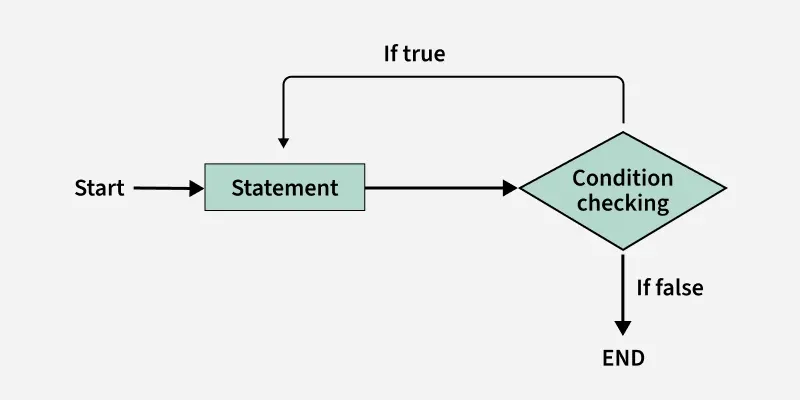
\includegraphics[width=0.85\linewidth]{Perulangan/do-while-flowchart.png}
      \caption{Alur eksekusi DO-WHILE Loop dalam Java}
      \label{fig:placeholder}
  \end{figure}
  \textbf{Sumber: }GeeksforGeeks - Java Loop
\end{frame}

% Section 5: Perbandingan Jenis Perulangan
\section{Perbandingan Jenis Perulangan}
\begin{frame}{Perbandingan FOR, WHILE, dan DO-WHILE}
  \begin{table}
    \footnotesize
    \begin{tabular}{p{0.3\textwidth}|p{0.2\textwidth}|p{0.2\textwidth}|p{0.2\textwidth}}
    \textbf{Kriteria} & \textbf{FOR} & \textbf{WHILE} & \textbf{DO-WHILE} \\
    \hline
    \rowcolor{lightgray}
    Pengecekan kondisi & Awal & Awal & Akhir \\
    \rowcolor{white}
    Jumlah eksekusi minimal & 0 & 0 & 1 \\
    \rowcolor{lightgray}
    Inisialisasi counter & Dalam statement & Diluar loop & Diluar loop \\
    \rowcolor{white}
    Cocok untuk & Iterasi diketahui & Iterasi tidak pasti & Minimal 1x eksekusi \\
    \rowcolor{lightgray}
    Contoh penggunaan & Array, deret & Input validation & Menu program \\
    \end{tabular}
    \caption{Perbandingan Jenis Perulangan dalam Java}
  \end{table}
\end{frame}

\begin{frame}[fragile]{Kapan Menggunakan Masing-masing Loop?}
  \vspace{-0.2cm}
  \begin{block}{FOR Loop}
    \begin{lstlisting}[basicstyle=\ttfamily\tiny]
// Ketika jumlah iterasi diketahui
for(int i = 0; i < array.length; i++) {
    System.out.println(array[i]);
}
    \end{lstlisting}
  \end{block}

  \vspace{-0.5cm}
  \begin{block}{WHILE Loop}
    \begin{lstlisting}[basicstyle=\ttfamily\tiny]
// Ketika jumlah iterasi tidak pasti
while(scanner.hasNextInt()) {
    int num = scanner.nextInt();
    // process number
}
    \end{lstlisting}
  \end{block}

  \vspace{-0.5cm}
  \begin{block}{DO-WHILE Loop}
    \begin{lstlisting}[basicstyle=\ttfamily\tiny]
// Ketika perlu eksekusi minimal sekali
do {
    System.out.print("Masukkan password: ");
    password = scanner.nextLine();
} while(!isValidPassword(password));
    \end{lstlisting}
  \end{block}
\end{frame}

% Section 6: Nested Loops
\section{Nested Loops}
\begin{frame}[fragile]{Konsep Nested Loops}
  \begin{block}{Definisi}
    Nested loops (perulangan bersarang) adalah perulangan yang berada di dalam perulangan lainnya.
  \end{block}
  
  \begin{exampleblock}{Contoh Program Nested FOR Loop}
    \begin{lstlisting}
public class NestedFor {
    public static void main(String[] args) {
        for(int i = 0; i < 3; i++) {
            System.out.println("Iterasi luar: " + i);
            
            for(int j = 0; j < 2; j++) {
                System.out.println("  Iterasi dalam: " + j);
            }
        }
    }
}
    \end{lstlisting}
  \end{exampleblock}
\end{frame}

\begin{frame}[fragile]{Nested Loops untuk Pola Bintang}
  \vspace{-0.2cm}
  \begin{exampleblock}{Contoh Program Segitiga Bintang}
    \begin{lstlisting}[basicstyle=\ttfamily\scriptsize]
public class PolaBintang {
    public static void main(String[] args) {
        int tinggi = 5;
        
        for(int i = 1; i <= tinggi; i++) {
            for(int j = 1; j <= i; j++) {
                System.out.print("*");
            }
            System.out.println();
        }
    }
}
    \end{lstlisting}
  \end{exampleblock}

  \vspace{-0.55cm}
  \begin{block}{Output Program}
    \colorbox{gray!20}{
      \parbox{0.9\textwidth}{
        \texttt{\tiny *\\[-5pt]
        **\\[-5pt]
        ***\\[-5pt]
        ****\\[-5pt]
        *****}
      }
    }
  \end{block}
\end{frame}

% Section 7: Loop Control Statements
\section{Loop Control Statements}
\begin{frame}[fragile]{BREAK Statement}
\vspace{-0.25cm}
  \begin{block}{Fungsi BREAK}
  \vspace{-0.2cm}
    Menghentikan eksekusi loop secara paksa dan keluar dari loop.
  \end{block}
  \begin{exampleblock}{Contoh Program BREAK dalam Loop}
    \begin{lstlisting}[basicstyle=\ttfamily\tiny]
public class BreakExample {
    public static void main(String[] args) {
        for(int i = 0; i < 10; i++) {
            if(i == 5) {
                break;  // Keluar loop ketika i = 5
            }
            System.out.println("i = " + i);
        }
        System.out.println("Loop selesai");
    }
}
    \end{lstlisting}
  \end{exampleblock}

  \vspace{-0.5cm}
  \begin{block}{Output Program}
  \vspace{-0.3cm}
    \colorbox{gray!20}{
      \parbox{0.9\textwidth}{
        \texttt{\tiny i = 0\\[-5pt]
        i = 1\\[-5pt]
        i = 2\\[-5pt]
        i = 3\\[-5pt]
        i = 4\\[-5pt]
        Loop selesai}
      }
    }
  \end{block}
\end{frame}
\begin{frame}[fragile]{CONTINUE Statement}
\vspace{-0.25cm}
  \begin{block}{Fungsi CONTINUE}
  \vspace{-0.2cm}
    Melewati iterasi saat ini dan melanjutkan ke iterasi berikutnya.
  \end{block}
  \begin{exampleblock}{Contoh Program CONTINUE dalam Loop}
    \begin{lstlisting}[basicstyle=\ttfamily\tiny]
public class ContinueExample {
    public static void main(String[] args) {
        for(int i = 0; i < 10; i++) {
            if(i % 2 == 0) {
                continue;  // Lewati bilangan genap
            }
            System.out.println("i = " + i);
        }
    }
}
    \end{lstlisting}
  \end{exampleblock}

  \vspace{-0.5cm}
  \begin{block}{Output Program}
  \vspace{-0.3cm}
    \colorbox{gray!20}{
      \parbox{0.9\textwidth}{
        \texttt{\tiny i = 1\\[-5pt]
        i = 3\\[-5pt]
        i = 5\\[-5pt]
        i = 7\\[-5pt]
        i = 9}
      }
    }
  \end{block}
\end{frame}

% Section 8: Enhanced FOR Loop
\section{Enhanced FOR Loop}
\begin{frame}[fragile]{Enhanced FOR Loop (For-Each)}
  \vspace{-0.2cm}
  \begin{block}{Konsep For-Each}
    \vspace{-0.2cm}
    Penyederhaan loop khusus untuk iterasi melalui array\\
    \scriptsize\textcolor{gray}{Konsep array akan dipelajari di Modul 10, ini hanya sebagai pengantar}
  \end{block}

  \vspace{-0.2cm}
  \begin{exampleblock}{Contoh Program For-Each dengan Array}
    \begin{lstlisting}[basicstyle=\ttfamily\scriptsize]
public class ForEachExample {
    public static void main(String[] args) {
        int[] numbers = {1, 2, 3, 4, 5, 6, 7, 8, 9, 10};
        
        // Enhanced for loop
        for(int number : numbers) {
            System.out.println(number);
        }
    }
}
    \end{lstlisting}
  \end{exampleblock}

  \vspace{-0.5cm}
  \begin{block}{Keunggulan For-Each}
  \vspace{-0.2cm}
    \begin{itemize}
      \item \scriptsize Lebih sederhana dan mudah dibaca
      \item \scriptsize Tidak perlu mengelola index manual
      \item \scriptsize Tidak mungkin terjadi index out of bounds (index yang melebihi batas)
    \end{itemize}
  \end{block}
\end{frame}

% Section 9: Best Practices
\section{Best Practices}
\begin{frame}{Best Practices Penggunaan Loop}
  \begin{alertblock}{Tips dan Rekomendasi}
    \begin{itemize}
      \item \textbf{\scriptsize Pilih loop yang tepat} sesuai kebutuhan
      \item \textbf{\scriptsize Hindari infinite loops} dengan memastikan kondisi berakhir
      \item \textbf{\scriptsize Gunakan nama variabel yang bermakna} untuk counter
      \item \textbf{\scriptsize Minimalkan perhitungan dalam kondisi} loop
      \item \textbf{\scriptsize Gunakan enhanced for} ketika iterasi array
      \item \textbf{\scriptsize Hati-hati dengan nested loops}
    \end{itemize}
  \end{alertblock}
  
  \begin{block}{Kesalahan Umum}
    \begin{itemize}
      \item \scriptsize Lupa increment counter (loop tak berakhir)
      \item \scriptsize Kesalahan perhitungan satu angka
      \item \scriptsize Modifikasi counter dalam badan loop
      \item \scriptsize Loop bersarang yang terlalu dalam
    \end{itemize}
  \end{block}
\end{frame}

% Section 10: Latihan
\section{Latihan}
\begin{frame}{Latihan 1: Deret Fibonacci}
  \begin{block}{Soal 1: Deret Fibonacci}
    Buat program yang meminta input berupa integer positif n, kemudian menampilkan n suku pertama deret Fibonacci.
    
    \textbf{Rumus Fibonacci:}
    \begin{itemize}
      \item F(1) = 1
      \item F(2) = 1  
      \item F(n) = F(n-1) + F(n-2) untuk n \textgreater 2
    \end{itemize}
    
    \textbf{Contoh:} Input 7 → Output: 1, 1, 2, 3, 5, 8, 13
  \end{block}
\end{frame}

\begin{frame}{Latihan 2: Bilangan Prima}
  \begin{block}{Soal 2: Cek Bilangan Prima}
    Buat program yang meminta input berupa integer positif, kemudian menentukan apakah bilangan tersebut prima atau bukan.
    
    \textbf{Ciri bilangan prima:}
    \begin{itemize}
      \item Hanya habis dibagi 1 dan dirinya sendiri
      \item Bilangan \textgreater 1
      \item Contoh: 2, 3, 5, 7, 11, 13, ...
    \end{itemize}
    
    \textbf{Contoh:}
    \begin{itemize}
      \item Input 7 → Output: "7 adalah bilangan prima"
      \item Input 9 → Output: "9 bukan bilangan prima"
    \end{itemize}
  \end{block}
\end{frame}

\begin{frame}[fragile]{Latihan 3: Pola Segitiga Angka}
  \begin{block}{Soal 3: Segitiga Angka}
    Buat program yang meminta input berupa integer n, kemudian menampilkan pola segitiga angka seperti berikut:
    
    \textbf{Contoh n = 4\\Output:}
    \begin{verbatim}
1
12
123
1234
    \end{verbatim}
  \end{block}
\end{frame}

\begin{frame}{Latihan 4: Menghitung Faktorial}
  \begin{block}{Soal 4: Menghitung Faktorial}
    Buat program yang meminta input berupa integer positif n, kemudian menghitung dan menampilkan nilai n! (n faktorial).
    
    \textbf{Rumus Faktorial:}
    \begin{itemize}
      \item n! = 1 × 2 × 3 × ... × n
      \item 0! = 1 (menurut definisi)
      \item Tidak terdefinisi untuk bilangan negatif
    \end{itemize}
    
    \textbf{Contoh:}
    \begin{itemize}
      \item 5! = 5 × 4 × 3 × 2 × 1 = 120
      \item 0! = 1
    \end{itemize}
  \end{block}
\end{frame}

% Section 11: Kesimpulan
\section{Kesimpulan}
\begin{frame}{Kesimpulan}
  \begin{alertblock}{Inti Bab 7: Perulangan (Looping)}
    \begin{itemize}
      \item \textbf{3 jenis loop}: FOR, WHILE, DO-WHILE
      \item \textbf{FOR}: jumlah iterasi diketahui
      \item \textbf{WHILE}: kondisi kompleks
      \item \textbf{DO-WHILE}: eksekusi minimal sekali
      \item \textbf{Control}: BREAK (berhenti) dan CONTINUE (lewati)
      \item \textbf{Nested loops}: pola dan data multidimensi
      \item \textbf{Enhanced for}: iterasi array lebih mudah
    \end{itemize}
  \end{alertblock}
\end{frame}

% Section 12: Referensi
\section{Referensi}
\begin{frame}{Referensi}
  \begin{block}{Referensi:}
    \begin{itemize}
      \item \textbf{Modul Praktikum Algoritma dan Pemrograman - Modul 7}\\
            Departemen Matematika FSAD ITS
      \item \textbf{Oracle Java Tutorials - Control Flow Statements}\\
            \url{https://docs.oracle.com/javase/tutorial/java/nutsandbolts/flow.html}
      \item \textbf{GeeksforGeeks - Loops in Java}\\
            \url{https://www.geeksforgeeks.org/loops-in-java/}
    \end{itemize}
  \end{block}
\end{frame}

% Penutup
\begin{frame}[standout]
  \Huge \textbf{Terima Kasih} \\[1.5em]
  \Large Pertanyaan dan Diskusi
\end{frame}

\end{document}